\section{Psicosi acute brevi}

\subsection{Nosografia}

Nei sistemi nosografici attuali, le psicosi acute brevi hanno una loro
autonomia nosografica: sono psicosi distinte sia rispetto alla
schizofrenia, sia rispetto ai disturbi affettivi, sia rispetto ai
disturbi deliranti cronici.

Nell'ICD-10 questa autonomia è ribadita: non sono imparentate né con la
schizofrenia né con i disturbi cronici.

Nel TSM, pur mantenendo una loro autonomia nosografica, fanno parte
della macrocategoria ``schizofrenia e altri disturbi psicotici''.

\subsection{Definizione}

Le \textbf{psicosi acute brevi} (\textbf{PAB}) sono in gruppo alquanto
eterogeneo di \emph{disturbi psicotici endogeni non affettivi},
all'interno del quale sono raccolte diverse forme psichiatriche ad
eziologia variabile, tutte accumunate da due caratteristiche essenziali,
cioè l'\textbf{\emph{esordio acuto}} e la \textbf{\emph{breve durata}},
anche spontanea, che non va in genere oltre a qualche giorno o
settimana.

Per definizione, quindi, si può propriamente parlare di PAB quando si ha
un \textbf{quadro delirante e/o allucinatorio acuto}, dalla
\textbf{durata relativamente breve}, spesso \textbf{innescate da eventi
stressanti}, che si sviluppa in \textbf{assenza delle caratteristiche di
una personalità pre-morbosa schizoide o schizotipica}, avendo peraltro
una \textbf{prognosi favorevole}. Il paziente tipico affetto da PAB è
quindi un soggetto che non ha una personalità vicina alla schizofrenia,
ha in genere un'età che va dall'adolescenza sino ai 30-40 anni (più
avanzata rispetto alla schizofrenia), e sono soggetti del tutto
insospettabili, del tutto normali.

Va inoltre ricordato che quelle che oggi chiamiamo PAB sono in realtà
disturbi da sempre descritti in letteratura (ad esempio in Scandinavia
erano un tempo chiamate ``\emph{psicosi psicogene}'' per indicare
l'esordio scatenato da eventi stressanti) e che erano precedentemente
raccolti nel \textbf{disturbo schizofreniforme} proposto da Langfeld nel
1939.

\subsection{Langfield: disturbo schizofreniforme}

Langfeld, per definire le psicosi acute brevi coniò il termine di
\textbf{disturbo schizofreniforme}: disturbo simile alla schizofrenia
che però non è schizofrenia.

Tale denominazione diagnostica esiste ancora adesso ma è completamente
diversa dal concetto di Langfeld; \emph{\emph{attualmente}} infatti è
intesa come una diagnosi provvisoria di schizofrenia nella quale manca
il \emph{criterio temporale}, ossia che il quadro clinico deve
persistere per più di sei mesi.

Langfeld invece identifica come disturbo schizofreniforme quel disturbo
che presenti determinati elementi prognostici favorevoli, ossia elementi
che ci indirizzano verso la diagnosi di psicosi acuti brevi e che ci
facciano escludere la diagnosi di schizofrenia.

Tali elementi sono:

\begin{itemize}
\item
  \textbf{\emph{esordio acuto}}: anche la schizofrenia può insorgere
  acutamente, per processo, anche se le forme più gravi di schizofrenia
  sono l'esordio per sviluppo (lento, graduale.. ) -\textgreater{}
  esordio acuto: elemento favorevole;
\item
  \textbf{\emph{reattività}}: l'evidenziare un legame forte cronologico
  di causa-effetto tra un evento importante di vita e l'esordio della
  psicosi. Ovviamente anche quadri gravi, come alcune forme di
  schizofrenia, possono insorgere da un evento scatenante ma nelle
  psicosi acute brevi è fondamentale che ci sia questo legame;
\item
  \textbf{\emph{alterazioni affettive}:} movimenti affettivi molto
  evidenti, oscillazioni del tono dell'umore con instabilità affettiva.
  Una regola aurea della psicopatologia dice infatti che più elementi
  affettivi troviamo più la prognosi è favorevole. Ovviamente tale
  elemento può essere considerato \emph{controintuitivo}: tale
  alterazione affettiva è più impressionabile;
\item
  \textbf{\emph{alterazioni dello stato di coscienza}}: il fatto di
  un'alterazione più o meno grave dello stato di coscienza è un evento
  prognostico favorevole perché è più tipico di quadri affettivi.

\begin{itemize}
\item
  Alterazioni di tipo \emph{\emph{crepuscolare}} : il campo di coscienza
  è ristretto: quando abbiamo uno stato di coscienza integro normalmente
  esso è focalizzato su una sola azione ma nella mia mente ho la
  continua percezione di tutto ciò che mi circonda, avendo quindi un
  campo di coscienza molto ampio. Un restringimento del campo di
  coscienza è caratterizzato dal fatto che il campo di coscienza è
  focalizzato su un unico contenuto di coscienza.
\item
  Alterazioni di tipo \emph{\emph{confusionario}}: vi è una distruzione
  dei parametri spazio temporali ed elementi della realtà sono frammisti
  ad elementi deliranti allucinatori.
\end{itemize}

\item
  \textbf{\emph{assenza di sintomi negativi}}: i sintomi negativi sono i
  sintomi core della schizofrenia (apatia, abulia\ldots{}). Se noi
  ravvisiamo sintomi negativi forse dietro c'è un quadro schizofrenico;
\item
  \textbf{\emph{polimorfi sintomi positivi}}: i pazienti affetti da
  psicosi acute brevi sono affetti solo da sintomi positivi. Tali
  sintomi sono molto floridi, molto produttivi cioè presentano deliri
  cangianti (il paziente non costruisce un delirio sistematizzato ma ha
  deliri che vanno e vengono e vengono sostituiti da altri deliri: i
  contenuti cambiano di volta in volta anche rapidamente) e
  allucinazioni polisensoriali (possono coinvolgere tutti i canali
  sensoriali);
\item
  \textbf{\emph{buon adattamento premuroso}}: prima dell'esordio questi
  pazienti avevano un buon funzionamento. Nella schizofrenia ciò non
  avviene: il funzionamento avviene al di sotto dei livelli standard
  (personalità pre-morbosa).
\item
  \textbf{\emph{prognosi favorevole}}: a breve termine si ha remissione.
\end{itemize}

Domanda: oltre alla reattività del fattore stressante, vi sono altri
fattori di rischio? Sì, alcuni episodi sono legati a un basso QI: una
fragilità cognitiva indica meno risorse di adattamento.

Caso clinico: \emph{un ragazzo di 20 anni giunge all'osservazione del
medico di famiglia e poi dello psichiatra, con un buon funzionamento
pre-morboso, fu trovato a letto, per mano ai genitori con alterazione di
tipo crepuscolare di coscienza (non voleva essere abbandonato dai
genitori altrimenti sarebbe successo qualcosa). Tale quadro è durato 48
ore per poi andare incontro a risoluzione completa, senza ricordare
nulla di cosa era successo.} ( N.B.: più è alterato lo stato di
coscienza, più è facile che l'episodio venga dimenticato)

\subsection{Esordio e decorso}

Essi sono disturbi psicotici che, come dice il termine stesso, tendono
ad avere una determinata durata nel tempo: sono \textbf{acute},
esordiscono rapidamente, nell'arco di pochi giorni, settimane e tendono
ad andare incontro a remissioni.

Hanno una modalità di decorso opposta ai disturbi deliranti cronici, i
quali esordiscono gradualmente e tendono a mantenersi nel tempo; il
delirio, infatti, tende ad avere un andamento centrifugo, ad espandersi
sempre di più.

Le psicosi acute brevi tendono ad insorgere rapidamente e sempre
rapidamente vanno incontro a remissione.

Questi quadri insorgono in assenza di caratteristiche pre-morbose di
tipo schizoide o schizotipico: non si innestano su tratti di personalità
appartenenti allo spettro schizofrenico, tant'è che generalmente il
quadro pre-morboso non lascia evidenziare elementi che ci indicano la
probabilità di insorgenza di una psicosi acuta breve.

Il paziente tipico affetto da PAB è quindi un soggetto che non ha una
personalità vicina alla schizofrenia, ha in genere un'età che va
dall'adolescenza sino ai 30-40 anni (più avanzata rispetto alla
schizofrenia), e sono soggetti del tutto insospettabili, del tutto
normali.

Esordio: solitamente presentano tale esordio acuto, \emph{improvviso},
anche se talvolta possono insorgere con sintomi acuti
\textbf{\emph{prodromici}}, che però passano inosservati: sono infatti
sintomi lievi, aspecifici (ansia, stanchezza, cambiamenti di umore,
depersonalizzazione, alterazioni anche repentine dell'umore, perplessità
ed alterazioni neuro-vegetative, in particolare l'insonnia) ma che mai
destano una particolare preoccupazione.

Dopo di che si passa alla \textbf{\emph{Fase di Stato}}, con deliri
immaginativi, allucinazioni, floridi e vari, non strutturati, molto
mutevoli e polimorfi, associati ad allucinazioni polisensoriali,
disorganizzazione ideativa e comportamentale, alterazioni dello stato di
coscienza (stato oniroide o crepuscolare) ed alterazioni dell'umore, che
può essere di tipo espansivo o di tipo depressivo. I pazienti inoltre
vivono con estrema partecipazione affettiva il loro mondo delirante,
spesso riferiscono di essere in comunicazione con Dio (umore espansivo),
altre volte riferiscono spavento e comunicazioni con demoni (umore
depresso), oppure hanno intense preoccupazione rivolte verso parenti ed
amici.

\begin{figure}[!ht]
\centering
	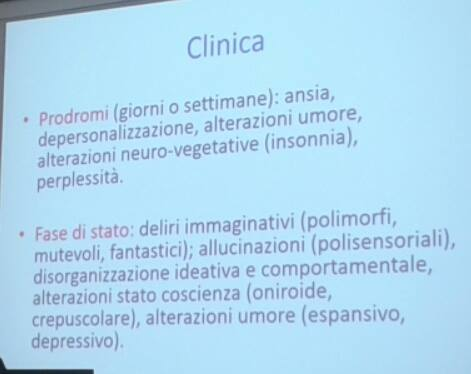
\includegraphics[width=0.9\textwidth]{09/image1.jpeg}
\end{figure}

La prognosi è generalmente favorevole, anche nell' evoluzione naturale
di questi disturbi, ossia anche senza trattamento farmacologico: tendono
ad andare incontro a remissione da sole.

Sono quadri molto importanti perché insorgono in modo drammatico
(sintomatologia accentuata) in persone assolutamente normali (inserite
nella società, con interessi e relazioni interpersonali\ldots{}) e
ovviamente il primo quesito che un medico si deve porre è una netta DD
con quadri più impegnativi.

In altri termini, se esercitiamo in guardia medica e vediamo un
paziente, giovane, con un quadro sintomatologico di deliri e
allucinazioni, dobbiamo pensare più a psicosi acute brevi piuttosto che
a un quadro schizofrenico o di psicosi affettiva.

\subsection{Sintomatologia}

Le psicosi acute brevi si caratterizzano per una \textbf{sintomatologia
positiva} (delirante, allucinogena) molto florida, acuta, difficilmente
quindi passano inosservate e spesso sono innescati da eventi stressanti:
si evidenzia quindi un rapporto tra lo stile di vita e l'insorgenza del
quadro psicotico.

\subsection{Incidenza}

Generalmente i pazienti presentano un'età compresa tra i 30 e i 40 anni.

Tali psicosi acute brevi rappresentano il 3\% dei ricoveri psichiatrici.

\subsection{Risoluzione}

La \emph{risoluzione avviene entro 3 mesi dall'esordio}, e può rimanere
un ricordo dell'esperienza delirante (più nello specifico, si è visto
che tanto più alterato è lo stato di coscienza, tanto meno i pazienti
hanno memoria degli episodi psicotici). La risoluzione è spesso brusca,
sebbene non manchino i casi in cui le PAB si risolvono attraverso delle
fluttuazioni sintomatologiche più graduali, e si deve tenere a mente che
la risoluzione delle PAB è spesso una ``\emph{risoluzione a ponte}'',
cioè il paziente va in remissione completa ma può avere delle recidive
(tanti più episodi si hanno, tanto maggiore è la probabilità di averne
di nuovi, e con una maggior frequenza), per cui il decorso è per
definizione remittente, ed 1/3 dei pazienti mantiene l'autonomia
nosografica (cioè continua ad avere attacchi di PAB), mentre nei
restanti 2/3 ``evolvono'' ad altre forme, soprattutto disturbo bipolare
o schizofrenia.

I criteri di Langfeld sono molto importanti per valutare e predire se il
paziente andrà verso la schizofrenia o verso altro.

Spesso però non è facile raccogliere l'anamnesi di un paziente non
riuscendo quindi bene ad intuire se il paziente presenta un ridotto
funzionamento pre-morboso: i quadri clinici talvolta possono essere
molto più complessi.

\emph{Se il quadro delirante non si risolve entro 3 mesi è difficile che
si risolva}, e in questo caso è opportuno rivalutare la diagnosi, perché
si tratta probabilmente di schizofrenia..

Caso clinico: \emph{ricovero di una ragazza di 19 anni che aveva
apparentemente un buon funzionamento pre-morboso, aveva una rete di
amici e un fidanzato. Fu ricoverata di urgenza per un quadro psicotico
acuto breve caratterizzato da una sintomatologia delirante allucinogena
(con allucinazioni visive soprattutto, a contenuto terrifico), uno stato
di angoscia e un'alterazione dello stato di coscienza. Tale quadro andrà
incontro a risoluzione in 15 giorni (con terapia farmacologica, quindi
non sappiamo se si sarebbe risolta senza). Lei riprese la vita
precedente anche se nel corso dei mesi, pur non presentando sintomi
psicotici, iniziò a perdere piano piano tutte le sue capacità,
diminuendo quindi il suo funzionamento. Nell'arco di 5-6 mesi ebbe un
altro episodio, molto meno florido, che andò anch'esso in remissione,
dopo il quale il suo declino diventò più evidente, tanto è che nell'arco
di 1 anno e mezzo perse gli amici, il fidanzato, non studiò più e non
uscì più di casa. Questo è stato identificato come un quadro
schizofrenico.}

\emph{Se avessimo indagato bene il pre-morboso della ragazza potevamo
notare degli atteggiamenti che ci potevano insospettire (lei viveva in
un ambito molto protetto, con poche amicizie dell'infanzia, viveva in un
paesino sperduto di montagna, il ragazzo era lo stesso da quando aveva
13 anni, l'attività scolastica era incentrata su uno studio giorno e
notte per ottenere i minimi risultati. }

\emph{Domanda:} vi è familiarità? Sì. Essa è un aspetto molto importante
da indagare, soprattutto per riuscire ad inquadrare il disturbo che vi
può essere dietro. Se un paziente viene da una famiglia di
schizofrenici, l'episodio di psicosi acuta breve può nascondere un
disturbo schizofrenico alla base.

\subsection{Diagnosi}

Dal punto di vista diagnostico le PAB non sono semplicissime da
riconoscere, nel senso che, se da un lato danno sintomi molto eclatanti,
con pazienti estremamente deliranti, dall'altro è anche vero che tali
quadri sono spesso sovrapponibili a quelli della schizofrenia in fase
produttiva, e la diagnosi di certezza può quindi essere posta solo su di
un piano longitudinale, cioè osservando l'evoluzione della psicosi nel
tempo, e \emph{la diagnosi differenziale è essenziale dal punto di vista
prognostico}, perché le PAB hanno una \textbf{prognosi molto buona}, in
quanto vanno incontro a remissioni completa e non lasciano
compromissioni, mentre per la schizofrenia la prognosi è scarsa, perché
difficilmente si risolve e anche in remissione lascia spesso una marcata
compromissione del funzionamento del soggetto.

\subsection{DD}

Caso clinico: \emph{siamo laureati da due mesi e siamo in servizio come
guardie mediche, soli e lontani dal ps. Ci arriva un paziente di 18 anni
che due ore prima si presenta con un quadro di deliri e allucinazioni,
angosciato, con alterazione di stato di coscienza di tipo confusonirico
(non sa dove si trova\ldots{}). }

\emph{Possiamo fare un \emph{tossicologico} per vedere se alla base non
vi è una patologia psichiatrica ma un quadro di abuso di sostanze, anche
se non è detto che con un tossicologico negativo si possano escludere
questi quadri (esempio la ketamina che non risulta positiva al test).}

\emph{Con un tossicologico negativo, possiamo intraprendere una DD con
disturbi neurologici quali l'epilessia temporale e in tal caso faremo un
\emph{EEG}.}

\emph{Se l'EEG è negativo, possiamo fare anche una \emph{TAC}. Se anche
essa è negativa ci indirizziamo sempre di più verso una patologia
psichiatrica (è una personalità pre-morbosa? Dobbiamo indagare le
alterazioni affettive, lo stato di coscienza, se vi sono stati eventi
stressigeni precedenti\ldots{}).}

L'importante è differenziare le psicosi acute brevi dagli
\textbf{stati dissociativi}, i quali possono presentarsi con alterazioni
di coscienza di tipo crepuscolare. Quello che ci permette tale DD, è la
presenza di una personalità pre-morbosa di tipo dissociativo,
istrionico. La differenziazione purtroppo è molto difficile, viste le
similarità. Molti quadri che noi psichiatri occidentali inquadriamo come
psicosi acute breve, sono influenzati dalla nostra cultura; culture ad
esempio provenienti dall'Africa, rispondono a eventi stressigeni con
quadri dissociativi. 

\subsection{Trattamento}

I pazienti con psicosi acuta breve vengono trattati con antipsicotici.
Possono essere trattati anche con altri farmaci in base al quadro verso
il quale possono revertare negli episodi futuri. Potremmo quindi dare
stabilizzatori dell'umore (per curare un sospetto di quadro bipolare),
antidepressivi (se sospettiamo una depressione psicotica) etc\ldots{}

Non è una costante che, dopo un primo episodio di psicosi acuta breve,
se ne ripresentino altri benché più episodi vi sono nell'arco della
vita, più è possibile che ve ne siano altri.

La terapia antipsicotica, infatti, viene effettuata per 1 anno, se vi è
stato un unico episodio; se gli episodi sono stati 2, viene mantenuta
per 5 anni; se gli episodi sono stati 3 o più, la terapia viene
effettuata tutta la vita. Benché i quadri siano autorisolvibili, la
terapia viene effettuata per tutta la vita sia per prevenire la
re-insorgenza del quadro sia poiché non siamo certi che i quadri si
ripresentino nello stesso modo, ma potrebbero presentare quadri più
gravi.

\subsection{Altre forme psicotiche brevi}

I \textbf{disturbi psicotici brevi}, inclusi nel gruppo dei disordini
associati alla schizofrenia, sono suddivisibili in
\textbf{\emph{disturbo psicotico breve propriamente detto}} e
\textbf{\emph{disturbo schizofreniforme}}: il disturbo psicotico breve
p.d. è un quadro che dura meno di un mese, ed ha caratteristiche per il
resto sovrapponibili a quelle delle PAB, mentre il disturbo
schizofreniforme è un disturbo del tutto simile alla schizofrenia, ma
che dura meno di 6 mesi, ha anche sintomi negativi e non è escluso che
recidivi o diventi schizofrenia conclamata.
